% Chapter 1
%----------------------------------------------------------------------------------------------------------
\chapter{Single photoionization and resonance identification of S$^{8+}$}
% Main chapter title
\label{cha:sulphur} 
% For referencing the chapter elsewhere, use \ref{Chapter1} 
\lhead{Chapter 5. \emph{Photoionization of} S$^{8+}$} 
% This is for the header on each page - perhaps a shortened title
%----------------------------------------------------------------------------------------------------------

                           %                                              %
                          %%%                                    %%%
       %%%%%%%%%%      SECTION     %%%%%%%%%%
                          %%%                                    %%%
                           %                                             %
                           
\section{Introduction}\label{sec:sul_intro}
Now that we have discussed appropriate methods for generating accurate wavefunctions to describe the atomic target, we can avail of them to look at specific systems. Our aim is to implement these wavefunctions into the $R$-matrix method, as described in Chapter \ref{cha:rmatrix}, to compute atomic transitions that are required in a range of astrophysical and plasma applications.

The ions under investigation in this Chapter, S$^{8+}$ (S {\sc ix}) and S$^{9+}$ (S {\sc x}), have received much interest in recent years due to their astrophysical importance, and crucial scientific development has laid the foundations for line emission identifications of S {\sc x}. Examples of such identifications include early observations \cite{1965AnAp...28..755T}, laser produced plasmas in theta pinch experiments \cite{1973PhyS....8..244F, 1987PhyS...36...80F, 1966ApJ...144..435D, 1967ApJ...149..451D}, and more recently, beam-foil techniques \cite{1999PhyS...59..355K}. These important lines are visible in both the UV and soft X-Ray regimes of the electromagnetic spectrum, the latter exclusively arising from transitions of electrons occupying the $n = 3$ shells and in particular, transitions involving the ground state 2s$^2$2p$^3$ ($^4$S$_{3/2}^{\rm o}$). Additional S {\sc x} lines have also been observed spectroscopically in the nearby F-type star Procyon \cite{0004-637X-762-1-53} by instruments on board the Chandra satellite \cite{2000SpiE.4012...81B} as well as in the solar corona above an active region and within the quiet sun \cite{2003ApJ...582.1162M, 2012A&A...537A..38D}, through instruments on board Hinode EIS \cite{2007SoPh..243...19C} and also SOHO \cite{1995SoPh..162....1D}. Such observations are investigated with great scrutiny by modern laboratory techniques using the electron beam ion trap resulting in excellent agreement \cite{2014ApJ...788...25B, 2014ApJS..215....6T}.

For the S$^{9+}$ system there have been a number of publications pertaining to the generation of electron-impact excitation data. Initially \citet{2000ADNDT..76..176B} included only those target levels within the $n = 2$ complex plus one additional configuration, 2s$^{2}$2p$^{2}$3s. Then in 2003, \citet{2003ADNDT..85..169B} extended this work to include all $n = 3$ levels resulting in 34 $LS\pi$ coupled target states using the distorted wave approximation. The most sophisticated work to date was published in 2011 by \citet{2011A&A...533A..87L} who included configurations encompassing 84 levels within the $n = 3$ complex and implementing the intermediate-coupling frame transformation ({\sc icft}) $R$-matrix method. While we are not directly concerned with the electron scattering process, it is clear that the inclusion of all $n = 3$ orbitals and associated target levels is of major importance within our calculation. A consequence of this allows us to incorporate additional correlation when describing all scattering wavefunctions. Despite the lack of photoionization cross-sections within an intermediate coupling scheme available via the Opacity Project, calculations have been carried out elsewhere by Badnell et al. \cite{2005MNRAS.360..458B}. The data is available for download from the OPEN-ADAS compilation, thus providing comparable results. However, only resonance-free partial contributions to each target state are available, so the comparison is limited to background cross-Section only. A much more sophisticated evaluation of level resolved photoionization cross-sections is therefore required in order to benchmark results for appropriate plasma physics diagnostics in non-local thermodynamic equilibrium (NLTE) approximation calculations.

We express the photoionization process for the lowest five initial states of the S$^{8+}$ ion as,
\begin{eqnarray}\label{eq:sul_process}
& h\nu + \text{S}^{8+}~  [2s^22p^4]_{\rm J}  \longrightarrow ~ \text{S}^{9+}~ [2s^x2p^{3+y}3l^z + e^-] \nonumber \\ 
&  \searrow ~~~~ \nearrow\\ \nonumber
& (\text{S}^{8+})^*~ [2s^22p^3nd, 2s2p^4np, nf]
\end{eqnarray} 
where the electron is ejected through one of its channels provided it is open. The process can occur directly (along the top arrow) to leave the target and electron complex, or via a more indirect route which excites the S$^{8+}$ ion to some resonant state before the ejection of a photoelectron into the continuum. These autoionizing states are discussed and identified later in Section \ref{sec:sul_results} of this Chapter using appropriate techniques. This process is calculated for transitions of the nature $J=2, 1$ and $\Delta J = 0, \pm 1$ with the exception of $\Delta J  = 1$ for $J = 0$, allowing for change in parity to be conserved between initial and final states and the selection rules to be adhered, described in Section \ref{sec:many_selection}. The target  S$^{9+}$ can be simplified to the following constraints; $x+y+z = 2$ and $z\leq 1$ for $l = s, p, d$, which will be discussed in greater detail within Section \ref{sec:sul_target}.

\begin{table}[hbt]
\footnotesize
\begin{center}
\begin{tabular}{@{}        l r c r     |      l r c r        @{}}
\toprule
\multicolumn{1}{c}{$nl$} & \multicolumn{1}{c}{$c_{jnl}$} & \multicolumn{1}{c}{$I_{jnl}$} & \multicolumn{1}{c}{$\zeta_{jn}$} & \multicolumn{1}{c}{$nl$} & \multicolumn{1}{c}{$c_{jnl}$} & \multicolumn{1}{c}{$I_{jnl}$} & \multicolumn{1}{c}{$\zeta_{jn}$} \\  

\toprule
    %                                        &                   &     &                    &       &                   &    & \\
    \multicolumn{1}{c}{1s} & 0.95941    & 1 & 15.63090   & 3s  & 0.21735   & 1 & 12.05049\\     
                                            & 0.02266    & 1 & 26.59100   &       & --1.05970 & 2 & 5.00069 \\  
                                            & 0.00360    & 2 & 7.05116     &       & 1.53459   & 3 & 3.73297 \\                                                                    
                                            & 0.02453    & 2 & 13.23750   &       &                  &     & \\
                                            & --0.00197  & 2 & 6.05344     & 2p & 0.48450   & 2 & 6.67108\\
                                            &                    &    &                    &       & 0.08978   & 2 & 10.59010  \\
    \multicolumn{1}{c}{2s} & --0.29633  & 1 & 15.63090  &       & 0.44221   & 2 & 5.62582\\  
                                            & --0.00138  & 1 & 26.59100  &       & 0.00279   & 2 & 20.93410\\                                                                                                                                   
                                            & 0.19810    & 2 & 7.05116    &       &                  &     & \\   
                                            & --0.16315  & 2 & 13.23750  & 3p  & 0.59734   & 2 & 6.35642\\ 
                                            & 0.95388    & 2 & 6.05344    &         & --1.16636 & 3 & 3.47094 \\ 
                                            &                    &    &                   &       &                  &     & \\       
                                            &                    &    &                   &  3d  & 1.00000   & 3 & 3.54124\\
 %                                          &                   &     &                    &       &                   &    & \\      

\bottomrule
 \end{tabular}
  \caption{Orbital parameters for the optimized $n = 3$ orbitals of the radial form (\ref{eq:many_boundorbs}) generated using the computer package \protect{\sc{civ3}}. These orbitals are included alongside the existing Hartree-Fock orbitals of \citet{1974ADNDT..14..177C}. \label{tab:sul_orbitals}}
 \end{center}
\end{table}

%%%%%%%%%% TABLE %%%%%%%%%%%%%

\begin{table}[hbt]
\footnotesize
\begin{center}
\begin{tabular}{@{} l *4c c *3c @{}}
\toprule

\multicolumn{1}{c}{Index} & \multicolumn{1}{c}{Config.} & \multicolumn{1}{c}{Spec.} & \multicolumn{1}{c}{\textit{Martin}} & \multicolumn{1}{c}{\textit{Present}} &  \multicolumn{1}{c}{$\%$ Change} & \multicolumn{1}{c}{\textit{Liang}} & \multicolumn{1}{c}{\textit{Bhatia}} &  \multicolumn{1}{c}{\textit{Fischer}}    \\

\toprule

       \multicolumn{1}{c}{1} & 2s$^22$p$^3$ & $^4$S$^{\rm o}_{3/2}$ & 0.0000 & 0.0000 & 0.00 & 0.0000 & 0.0000 & 0.0000\\
       \multicolumn{1}{c}{2} & -- & $^2$D$^{\rm o}_{3/2}$ & 0.7513 & 0.7813 & 3.84 & 0.7929 & 0.7963 & 0.7568\\
       \multicolumn{1}{c}{3} & -- & $^2$D$^{\rm o}_{5/2}$ & 0.7618 & 0.7973 & 4.45 & 0.8101 & 0.8079 & 0.7681\\
       \multicolumn{1}{c}{4} & -- & $^2$P$^{\rm o}_{1/2}$ & 1.1571 & 1.1628 & 0.49 & 1.1932 & 1.1944 & 1.1597\\
       \multicolumn{1}{c}{5} & -- & $^2$P$^{\rm o}_{3/2}$ & 1.1738 & 1.1812 & 0.63 & 1.2131 & 1.2119 & 1.1765\\
       \multicolumn{1}{c}{6} & 2s2p$^4$ & $^4$P$_{5/2}$ & 3.4488 & 3.4403 & --0.25 & 3.4966 & 3.4954 & 3.4608\\
       \multicolumn{1}{c}{7} & -- & $^4$P$_{3/2}$ & 3.5117 & 3.4995 & --0.35 & 3.5593 & 3.5608 & 3.5239\\
       \multicolumn{1}{c}{8} & -- & $^4$P$_{1/2}$ & 3.5438 & 3.5317 & --0.34 & 3.5933 & 3.5942 & 3.5557\\
       \multicolumn{1}{c}{9} & -- & $^2$D$_{3/2}$ & 4.7452 & 4.8149 & 1.45 & 4.8730 & 4.8739 & 4.7647\\
       \multicolumn{1}{c}{10} & -- & $^2$D$_{5/2}$ & 4.7465 & 4.8185 & 1.49 & 4.8771 & 4.8763 & 4.7660\\
       \multicolumn{1}{c}{11} & -- & $^2$S$_{1/2}$ & 5.5477 & 5.6076 & 1.07 & 5.6861 & 5.6864 & 5.5645\\
       \multicolumn{1}{c}{12} & -- & $^2$P$_{3/2}$ & 5.8038 & 5.9266 & 2.07 & 5.9722 & 5.9715 & 5.8300\\
       \multicolumn{1}{c}{13} & -- & $^2$P$_{1/2}$ & 5.8837 & 6.0032 & 1.99 & 6.0544 & 6.0545 & 5.9101\\
       \multicolumn{1}{c}{14} & 2p$^5$ & $^2$P$^{\rm o}_{3/2}$ & 9.0329 & 9.1913 & 1.72 & 9.2852 & 9.2860 & 9.0635\\
       \multicolumn{1}{c}{15} & -- & $^2$P$^{\rm o}_{1/2}$ & 9.1343 & 9.2933 & 1.71 & 9.3900 & 9.3914 & 9.1650\\                                                                                           
       \multicolumn{1}{c}{16} & 2s$^2$2p$^23$s & $^4$P$_{1/2}$ & 19.0223 & 19.0677 & 0.24 & 18.9961 & 18.9959 & 19.0238\\
       \multicolumn{1}{c}{17} & -- & $^4$P$_{3/2}$ & 19.0674 & 19.1073 & 0.21 & 19.0380 & 19.0379 & 19.0660\\
       \multicolumn{1}{c}{18} & -- & $^4$P$_{5/2}$ & 19.1224 & 19.1648 & 0.22 & 19.0981 & 19.0979 & 19.1226\\       
       \multicolumn{1}{c}{19} & -- & $^2$P$_{1/2}$ & 19.2560 & 19.3011 & 0.23 & 19.2446 & 19.2445 & 19.2535\\       
       \multicolumn{1}{c}{20} & -- & $^2$P$_{3/2}$ & 19.3234 & 19.3698 & 0.24 & 19.3163 & 19.3161 & 19.3221\\       
       \multicolumn{1}{c}{21} & -- & $^2$D$_{5/2}$ & 19.6846 & 19.7480 & 0.32 & 19.6882 & 19.6881 & 19.6950\\
        \multicolumn{1}{c}{22} & -- & $^2$D$_{3/2}$ & 19.6768 & 19.7501 & 0.37 & 19.6907 & 19.6905 & 19.6924\\
        \multicolumn{1}{c}{23} & 2s$^2$2p$^2$3p & $^2$S$_{1/2}$ & -- & 19.9383 & -- & 19.8772 & 19.8771 & 19.8971\\ 
        \multicolumn{1}{c}{24} & -- & $^4$D$_{1/2}$ & -- & 20.0208 & -- & 19.9500 & 19.9499 & 19.9770\\
        \multicolumn{1}{c}{25} & -- & $^4$D$_{3/2}$ & -- & 20.0423 & -- & 19.9719 & 19.9718 & 19.9993\\
        \multicolumn{1}{c}{26} & -- & $^4$D$_{5/2}$ & -- & 20.0805 & -- & 20.0119 & 20.0118 & 20.0389\\
        \multicolumn{1}{c}{27} & -- & $^4$P$_{1/2}$ & -- & 20.1368 & -- & 20.0652 & 20.0651 & 20.0927\\
        \multicolumn{1}{c}{28} & -- & $^4$D$_{7/2}$ & -- & 20.1320 & -- & 20.0659 & 20.0741 & 20.0902\\
        \multicolumn{1}{c}{29} & -- & $^4$P$_{3/2}$ & -- & 20.1465 & -- & 20.0742 & 20.1103 & 20.1002\\
        \multicolumn{1}{c}{30} & -- & $^4$P$_{5/2}$ & -- & 20.1804 & -- & 20.1104 & 20.2001 & 20.1344\\        
\bottomrule
 \end{tabular}
 \caption{Target state energies (in eV) for the lowest 30 fine-structure levels of the target ion S$^{9+}$ relative to the $^4$S$^{\rm o}_{3/2}$ ground state. The column header \textit{Present} represents our current {\sc bprm} calculation, \textit{Martin} are the observed values currently available in the NIST database \citep{1990JPCRD..19..821M}, \textit{Liang} are the electron-impact excitation energies from \cite{0004-637X-762-1-53}, \textit{Bhatia} are those from \cite{2003ADNDT..85..169B} and \textit{Fischer} the structure calculation of \cite{2004ADNDT..87....1F}. The $\%$ change between our \textit{Present} results and \textit{Martin} has also been listed between each level. \label{tab:sul_energy}}
 \end{center}
\end{table}



\begin{table}[t]
\footnotesize
\begin{center}
\begin{tabular}{@{} l *2c @{}}
\toprule

\multicolumn{1}{c}{Main} & \multicolumn{1}{c}{Additional}  \\
\multicolumn{1}{c}{CSFs} & \multicolumn{1}{c}{Correlation CSFs}  \\

\toprule
   %    \multicolumn{1}{c}{} &  \\
       \multicolumn{1}{c}{2s$^2$2p$^3$} & 2p$^4$ [3s, 3p, 3d] \\
        \multicolumn{1}{c}{2s2p$^4$} & 2s2p$^2$ [3s$^2$, 3p$^2$, 3d$^2$] \\
       \multicolumn{1}{c}{2p$^5$} & 2s2p$^2$ [3s3p, 3s3d, 3p3d] \\
          \multicolumn{1}{c}{2s$^2$2p$^2$ [3s, 3p, 3d]}   & 2s$^2$2p [3s$^2$, 3p$^2$, 3d$^2$] \\
           \multicolumn{1}{c}{2s2p$^3$ [3s, 3p, 3d]} & 2s$^2$2p [3s3p, 3s3d, 3p3d] \\
                    & 2p$^3$ [3s$^2$, 3p$^2$, 3d$^2$] \\
                    & 2p$^3$ [3s3p, 3p3d, 3s3d] \\
      %          \multicolumn{1}{c}{} &  \\           
\bottomrule
 \end{tabular}
 \caption{Presented is a list of configurations included in the structure calculation, where square brackets define the assignment of the outermost orbitals pertaining to a common core of 1s$^2$. Provided are 9 main CSF's describing the 215 J$\pi$ levels and 21 additional CSF's for the inclusion of extra correlation. \label{tab:sul_ci}}
 \end{center}
\end{table}

\begin{table}[t]
\footnotesize
\begin{center}
\begin{tabular}{@{} l *6c @{}}
\toprule
\multicolumn{1}{c}{} & \multicolumn{1}{c}{NIST} & \multicolumn{1}{c}{Gu} & \multicolumn{1}{c}{Zheng} & \multicolumn{1}{c}{{\sc mcdf}} & \multicolumn{1}{c}{{\sc top}base} & \multicolumn{1}{c}{\textit{Present}} \\
 \toprule
     %   \multicolumn{1}{c}{} &  & &  &  &  &  \\
       \multicolumn{1}{c}{IP}& 379.84 & 379.63 & 379.10 & 377.78 & 378.67& 381.09 \\
        \multicolumn{1}{c}{$\Delta$IP} & 0.00 & --0.22 & --0.75 & --2.07 & --1.17 & 1.25\\
  %      \multicolumn{1}{c}{} &  & &  &  &  &  \\  
\bottomrule
 \end{tabular}
 \caption{A comparison of the ionization potential (IP) of S$^{8+}$ for a variety of theoretical calculations and our \textit{Present} result, where IP given in eV. $\Delta$IP represents the change in the ionization potential between NIST and the theoretical results. \label{tab:sul_ip}}
 \end{center}
\end{table}

                           %                                              %
                          %%%                                    %%%
       %%%%%%%%%%      SECTION     %%%%%%%%%%
                          %%%                                    %%%
                           %                                             %
\section{Target model}\label{sec:sul_target}
The first step of the $R$-matrix calculation consists of defining a set of basis functions to describe the system after photoionization occurs, in this case, S$^{9+}$ with atomic number $Z=16$ and $N=7$ electrons. The wavefunctions we choose for this system are configuration-interaction expansions of Configuration State Functions (CSF's) built with an orthogonal orbital basis set, taking the form of equation (\ref{eq:many_boundorbs}), with optimized coefficients $c_{jnl}, I_{jnl}$ and $\zeta_{jnl}$ determined by minimizing the total energy of different atomic states. We therefore consider the theory as outlined in Subsection \ref{sec:many_ci} for obtaining configuration-interaction wavefunctions.

The $1s$, $2s$ and $2p$ orbitals are Hartree-Fock orbitals from \citet{1974ADNDT..14..177C} and the $n=3$ orbitals have been optimized using the computer package {\sc civ3} \cite{1975CoPhC...9..141H}, described in Section \ref{sec:many_civ3}. Optimization of the orbital parameters is performed in $LS$ coupling, however, the wavefunctions used to determine the calculated S$^{9+}$ energies are obtained by adding the operators of the {\sc bp} Hamiltonian from equations (\ref{eq:many_bp1}), (\ref{eq:many_bp2}) and (\ref{eq:many_bp3}), to the non-relativistic Hamiltonian. The optimization was then carried out by minimizing on the lowest lying energy levels of the 2p$^2$3$l$ quartet and doublet states ($^4$P for $l=0$, $^4$P$^{\rm o}$ for $l=1$ and $^2$P for $l=2$) respectively. The parameters $c_{jnl}$, $I_{jnl}$ and $\zeta_{jnl}$ adopted for each $n = 3$ orbital are provided in Table \ref{tab:sul_orbitals}.

Table \ref{tab:sul_energy} presents the energies in eV obtained from the current model for the 30 lowest-lying fine-structure levels of the S$^{9+}$ ion relative to the 2s$^{2}$2p$^{3}$ $^{4}$S$^{\rm{o}}_{3/2}$ ground state. The energies were calculated in $LSJ$ coupling and by incorporating all CSF's listed in Table \ref{tab:sul_ci}. We compare with a variety of other theoretical calculations, Liang et al. \cite{2011A&A...533A..87L}, Bhatia and Landi \cite{2003ADNDT..85..169B} and the {\sc mchf} structure approach of \citet{2004ADNDT..87....1F}, and finally the observational values provided by \citet{1990JPCRD..19..821M}. Also listed are the \% differences between our present values and the observed values, highlighting the excellent agreement found for all levels considered. An excellent comparison is also evident between all of the theoretical predictions with the {\sc mchf} values of Fischer closest in agreement to \citet{1990JPCRD..19..821M} as expected, since this evaluation includes all relativistic operators apart from the spin-spin interaction and a large configuration-interaction expansion. For higher lying levels not considered in Table \ref{tab:sul_energy}, a similar accuracy is found. 

Finally in Table \ref{tab:sul_ip}, we summarize the measurements of the S$^{8+}$ ionization potential currently available in the literature, and compare with the value obtained from our current model. Bi\'{e}mont et al. \cite{1999ADNDT..71..117B} performed a fitting to a proposed series expansion of the ionization potential along iso-electronic sequences between previous NIST results and that of Multi-Configuration Dirac-Fock ({\sc mcdf}) calculations, which has been outlined briefly in Subsection \ref{ssec:many_mchf}. NIST has since been updated with this current value. Work carried out by Gu \cite{2005ADNDT..89..267G} involves a Dirac-Coulomb-Breit Hamiltonian for solving the TISE and an extensive configuration-interaction calculation to represent the wavefunctions. Zheng et al. \cite{2002PhRvA..65e2510Z} consider a potential term to describe the weakest bound electron when solving the TISE with a non-relativistic Hamiltonian, and by further extending this to include relativistic corrections. The {\sc mcdf} result has been generated through the computer codes of Grant et al. \cite{1980CoPhC..21..207G}. The TOPbase value is the bound state threshold in $LS$ coupling. The final entry represents our current {\sc bprm} work of 381.10 eV which lies approximately 1.22 eV (or less than 1\%) above the observed NIST value. Overall, excellent agreement is evident between the range of various techniques.

Much deliberation has therefore gone into the preliminary stage of the work in order to limit computational resources needed for the photoionization calculations. After considering many models, we opted for a S$^{9+}$ basis set of 94 $LS\pi$ states which results in 215 $J\pi$ fine-structure levels. We present in Table \ref{tab:sul_ci} the 9 main CSF's that represent the S$^{9+}$ states with an additional 21 configurations of the configuration-interaction expansion accounting for internal, semi-internal and external correlation necessary for improving the wavefunctions. This approach has been described previously in Section \ref{sec:many_config}.

                           %                                              %
                          %%%                                    %%%
       %%%%%%%%%%      SECTION     %%%%%%%%%%
                          %%%                                    %%%
                           %                                             %
                           
\section{Results and discussions}\label{sec:sul_results}
To remain consistent with the wavefunction expansions obtained in the computer package {\sc civ3}, we use the same Hamiltonian operators and therefore employ the {\sc bprm} suite of computer codes described in Section \ref{sec:codes} and Subsection \ref{ssec:BP}. Within the $R$-matrix framework, we select $r=4.6$ Bohr radii allowing convergence of the bound orbitals at the boundary as a consequence of their description in Table \ref{tab:sul_orbitals}. A total of 20 basis functions are chosen to represent the continuum when solving the radial component of the TISE. When constructing the scattering wavefunctions defined by equation (\ref{eq:rmat_boundbasis}), and equation (\ref{eq:rmat_freebasis}), we allow for triple excitation of electrons from the base configuration 1s$^2$2s$^2$2p$^4$ into the remaining $n=3$ complex maintaining a closed 1s$^2$ core. This generates numerous configurations to describe each state of our system and therefore the exploitation of parallel processing is essential in distributing routines through a systematic approach. 


\begin{figure}[hbt]
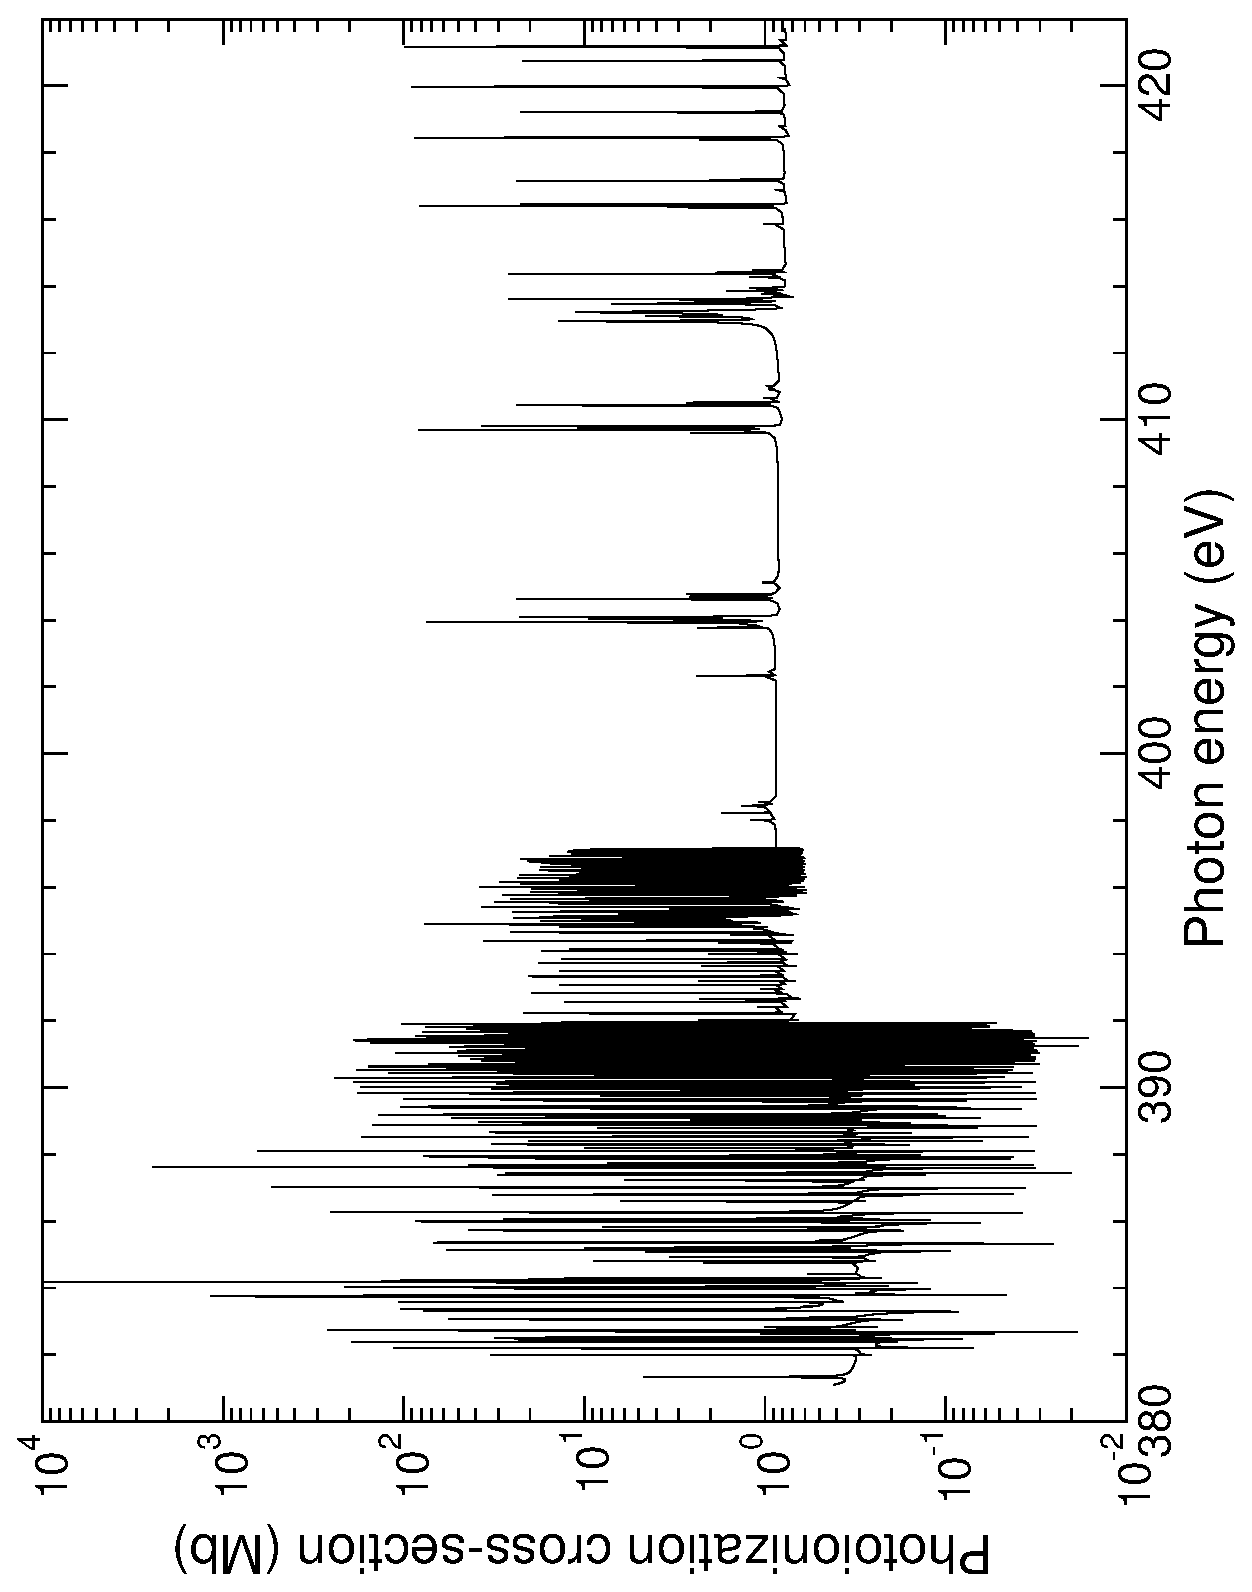
\includegraphics[scale=0.55, angle=-90]{Figures/Sulphur/ground/ground.eps}
\caption{Photoionization cross-section presented on a logarithmic scale in Mb as a function of photon energy in eV, between 380 - 420 eV. We show the fine-structure spectrum of the 2s$^2$2p$^4$ $^3$P$_2$ initial ground state to all allowed $J=1,2,3$ odd final states.\label{fig:sul_ground}}
\end{figure}

After obtaining initial and final state wavefunctions $\Psi_i$ and $\Psi_f$ from equations (\ref{eq:rmat_boundbasis}) and (\ref{eq:rmat_freebasis2}), and also the dipole moment contribution from the internal region defined in equations (\ref{eq:rmat_diplength}) and (\ref{eq:rmat_fullmatrix}), we then calculate the photoionization cross-section $\sigma_{PI}$ as defined in equation (\ref{eq:rmat_totphoto}). For each transition of interest, the photoionization cross-sections are computed for a range of photoelectron energies between 0 - 65 eV. This range for our spectrum is generated via a very fine energy mesh step size of $\approx 6.6 \times 10^{-5}$ eV to ensure that all complex resonance structures have been properly resolved. We also introduce the residual ion charge denoted as $z$ ($=Z-N$). Since length and velocity forms of the dipole approximations discussed in equation (\ref{eq:rmat_diplength}) and (\ref{eq:rmat_diplength}) are in good agreement, length gauge is considered to be the standard throughout. Up to 45 eV the difference in results is within 20\% and therefore all results are provided in the length gauge.

All photoionization scattering cross-sections have been computed within the intermediate coupling scheme, so that the ground and metastable states require dipole matrix transitions of the $J=2$ even state to allowed $J=1,2,3$ odd parity states (ground state $^3$P$_2$), the $J=1$ even state to $J=0,1,2$ odd states (first metastable $^3$P$_1$) and finally the $J=0$ even state to its only accessible final state of $J=1$ odd (second metastable $^3$P$_0$) due to the dipole selection rules.  We also present photoionization cross-sections for the next (lowest) two excited singlet states of the S$^{8+}$ ion, $^1$D$_2$ and $^1$S$_0$ respectively.

%
%%
%%%
%%%%
\begin{sidewaysfigure}
\centering
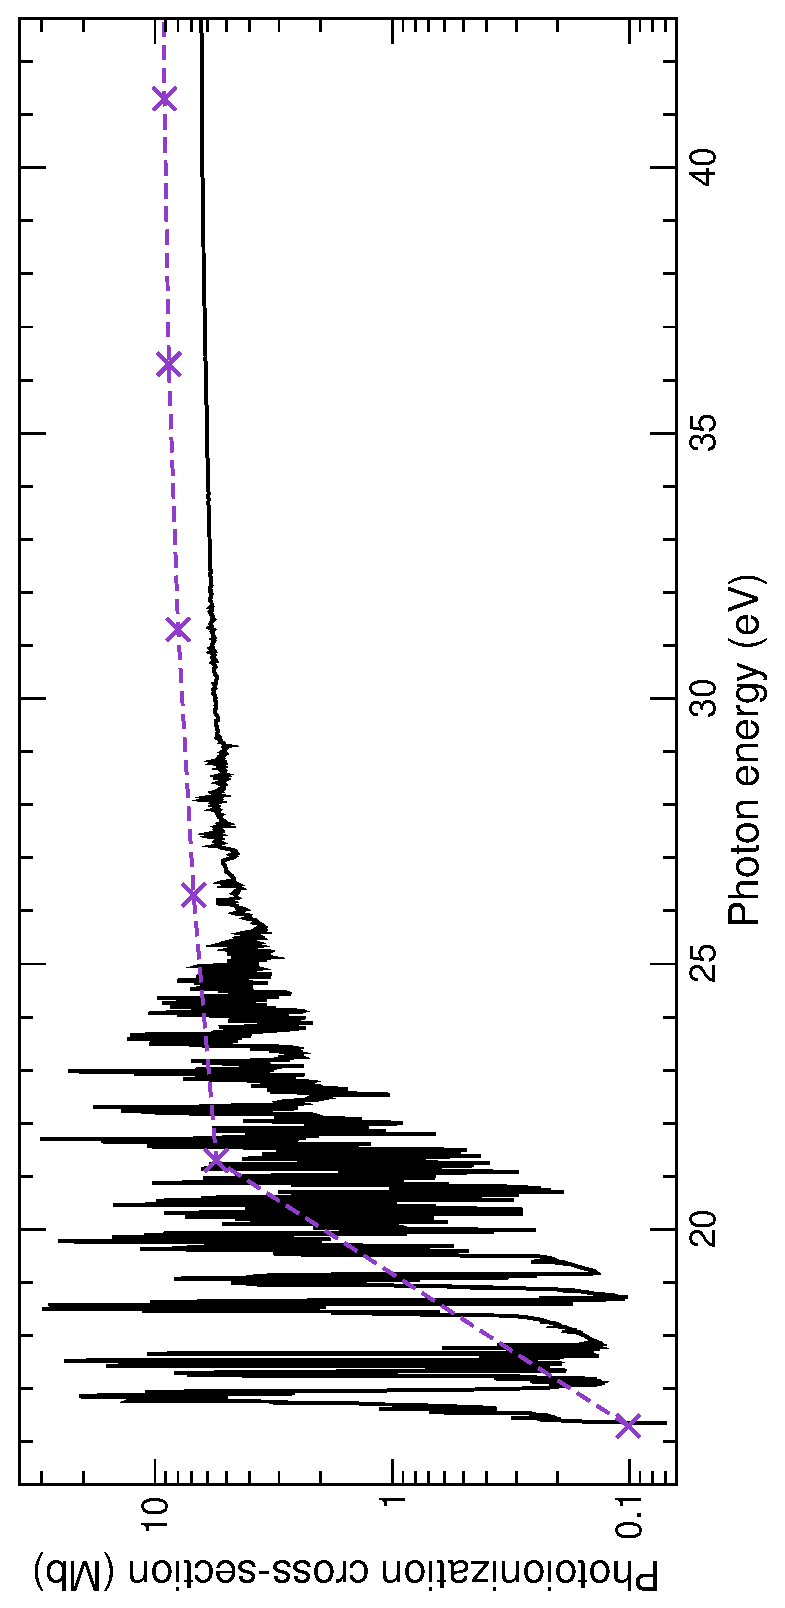
\includegraphics[scale=0.74, angle=-90]{Figures/Sulphur/meta/meta.eps}
\caption{Photoionization cross-sections presented on a logarithmic scale in Mb as a function of photon energy in eV for the remainder of metastable initial state transitions of the split $^3$P ground state, $^3$P$_1$ (top left) and $^3$P$_0$ (top right). The remaining figures display results for the lowest two excited initial singlet states, $^1$D$_2$ (bottom left) and $^1$S$_0$ (bottom right) to all allowed final states. \label{fig:sul_meta}}
\end{sidewaysfigure}

%
%%
%%%
%%%%
\begin{sidewaysfigure}
\centering
\includegraphics[scale=0.74, angle=-90]{Figures/Sulphur/target/target.eps}
\caption{Partial photoionization cross-sections on a logarithmic scale in Mb as a function of photon energy in eV. The contributions are transitions from the $^3$P$_2$ ground state to the lowest 4 final target levels $^4$S$^{\rm{o}}_{3/2}$ (top left), $^2$D$^{\rm{o}}_{3/2}$ (top right), $^2$D$^{\rm{o}}_{5/2}$ (bottom left), and $^2$P$^{\rm{o}}_{1/2}$ (bottom right) retaining to the 1s$^22$s$^2$2p$^3$ configuration through all allowed channels of the scattering electron. The circles represent results provided by the OPEN-ADAS website. \label{fig:sul_target}}
\end{sidewaysfigure}

We present first in Figure \ref{fig:sul_ground} the photoionization cross-section for the 2s$^2$2p$^4$ $^3$P$_2$ initial state of S$^{8+}$ on a logarithmic scale as a function of the photon energy in eV. All possible allowed final states of the S$^{9+}$ ion have been considered in producing this figure. Clearly visible are the Rydberg resonance series converging onto the target state thresholds. There is currently no direct data in the literature with which we can compare our total photoionization results with.

In Figure \ref{fig:sul_meta} we present similar figures representing photoionization cross-sections for the remaining metastable states $^3$P$_1$ (top left) and $^3$P$_0$ (top right) of the S$^{8+}$ ion, together with results for the first two excited singlet states $^1$D$_2$ (bottom left) and $^1$S$_0$ (bottom right) Again all allowed accessible levels of the final S$^{9+}$ ion are considered and care has been taken to ensure a proper delineation of the Rydberg resonance series converging onto the target state thresholds.

Generally, we require data from metastable and excited levels, as not every S$^{8+}$ ion will be in its ground state when considering specific astrophysical objects. In Section \ref{sec:sul_intro} we referred to a limited set of resonance-free partial photoionization cross-sections available for download from the OPEN-ADAS database \cite{2005MNRAS.360..458B}. In Figure \ref{fig:sul_target} we present partial photoionization cross-sections to the lowest four target level contributions of the S$^{9+}$ ion, $^4$S$^{\rm{o}}_{3/2}$ (top left), $^2$D$^{\rm{o}}_{3/2}$ (top right), $^2$D$^{\rm{o}}_{5/2}$ (bottom left), and $^2$P$^{\rm{o}}_{1/2}$ (bottom right) respectively, which correspond to transitions from the ground $^3$P$_2$ initial state of S$^{8+}$. Excellent agreement is evident for all four partial contributions across this low photoelectron energy range considered. The limited background values from OPEN-ADAS, although neglecting all resonance features, are in line with our base background photoionization cross-sections.

%
%%
%%%
%%%%
\begin{figure}[hbt]
\centering
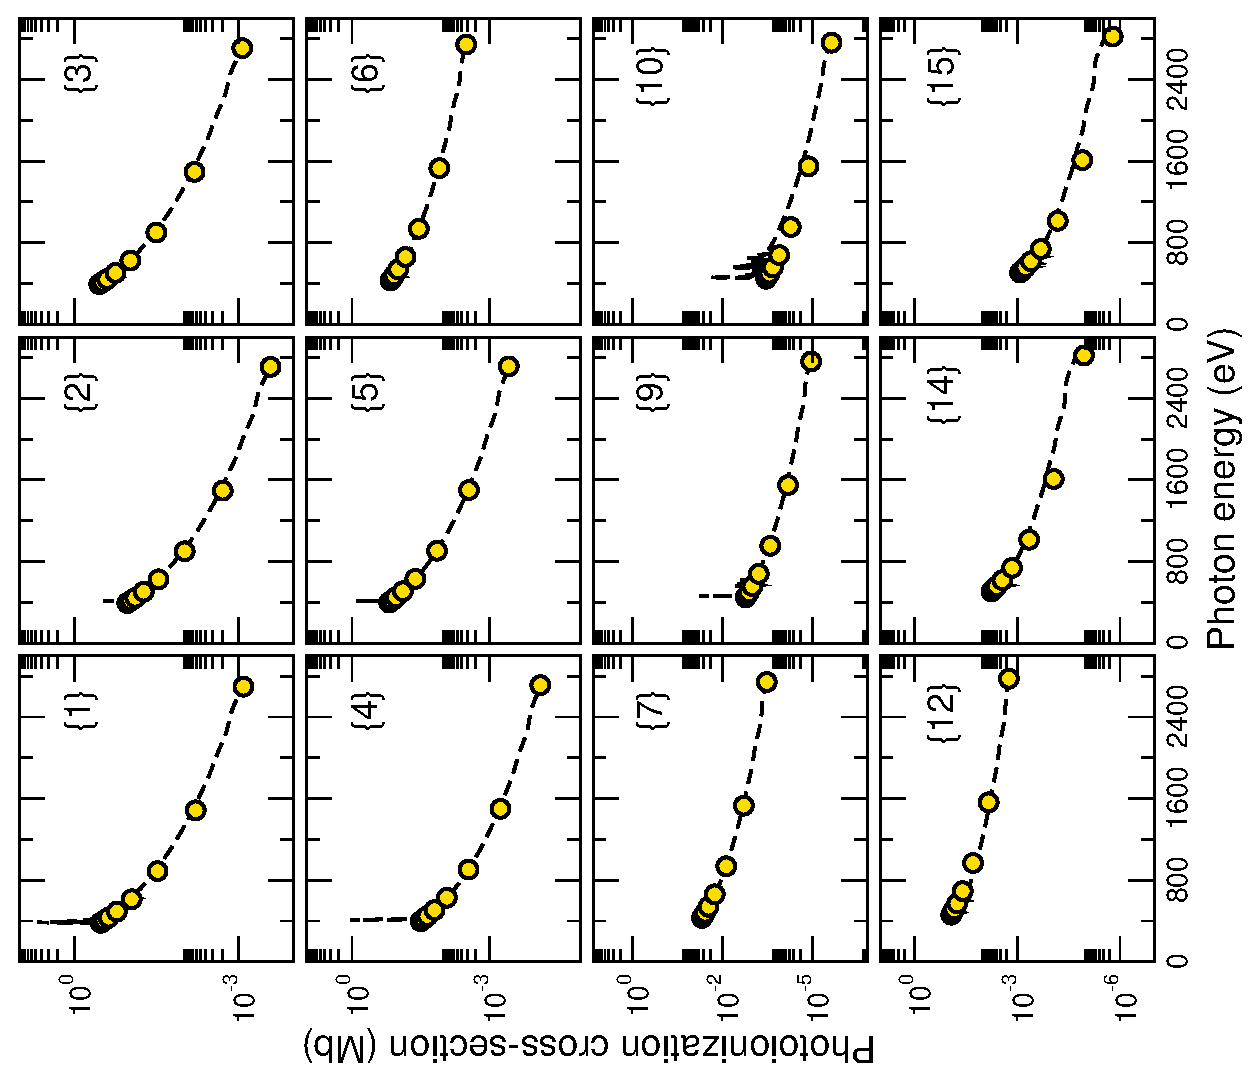
\includegraphics[scale=0.82, angle=-90]{Figures/Sulphur/open-adas/comparison1_new.eps}
\caption{Photoionization cross-sections presented on a logarithmic scale in Mb as a function of photon energy in eV up to 2,700 eV. Transitions are from the initial $^3$P$_2$ $\longrightarrow$ \{1\}, \{2\}, \{3\}, \{4\}, \{5\}, \{6\}, \{7\}, \{9\}, \{10\}, \{12\}, \{14\}, \{15\}. \label{fig:sul_adas2e}}
\end{figure}
%%%%
%%%
%%
%

%
%%
%%%
%%%%
\begin{figure}[hbt]
\centering
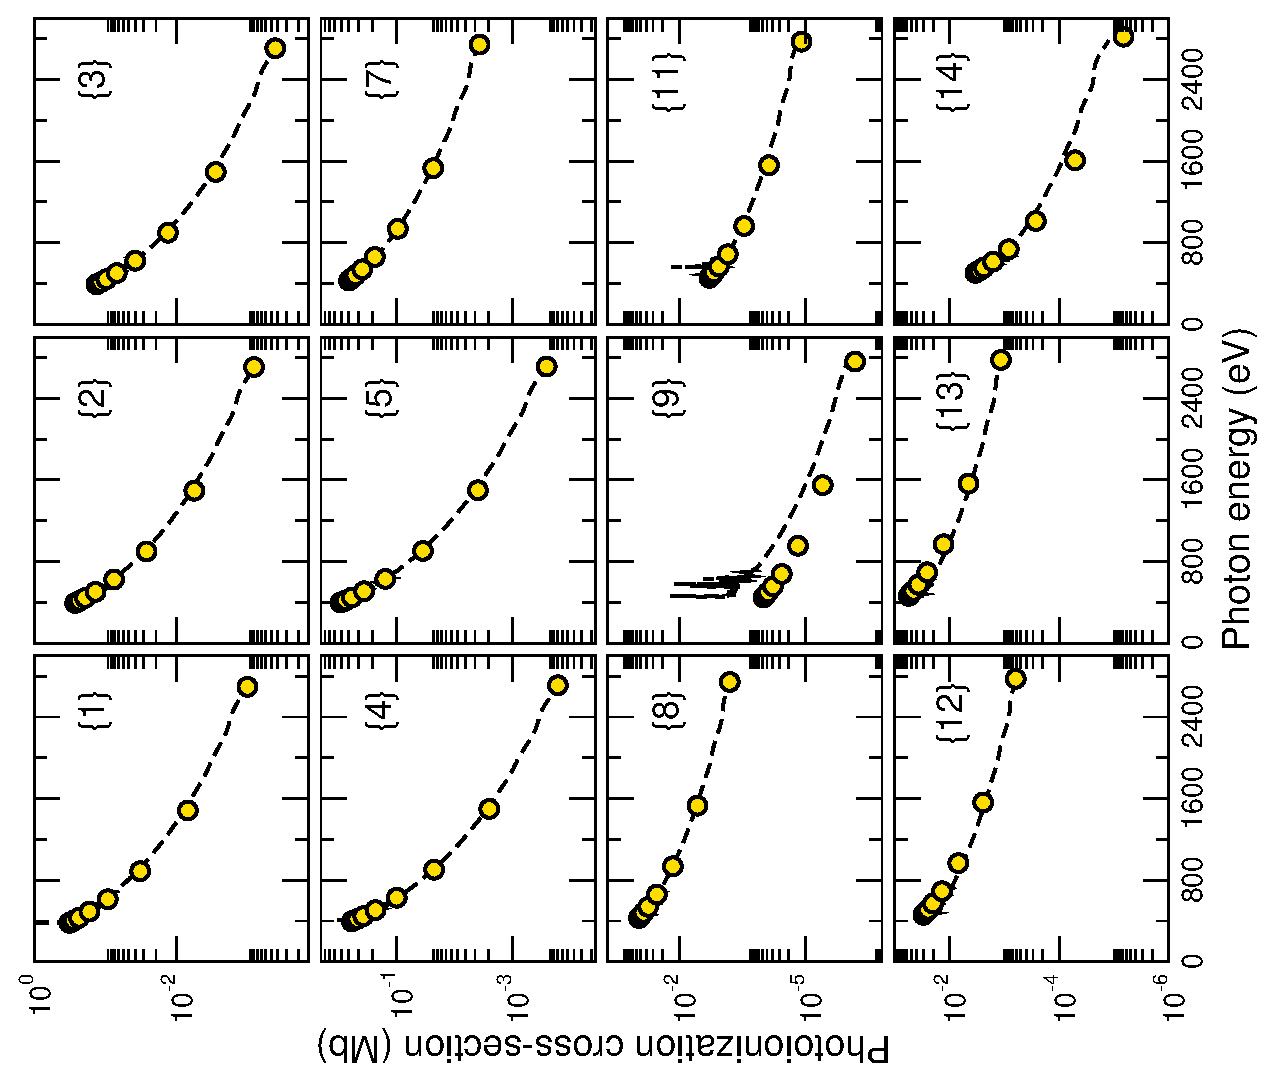
\includegraphics[scale=0.82, angle=-90]{Figures/Sulphur/open-adas/comparison2_new.eps}
\caption{Photoionization cross-sections presented on a logarithmic scale in Mb as a function of photon energy in eV up to 2,700 eV. Transitions are from the initial $^3$P$_1$ $\longrightarrow$ \{1\}, \{2\}, \{3\}, \{4\}, \{5\}, \{7\}, \{8\}, \{9\}, \{11\}, \{12\}, \{13\}, \{14\}. \label{fig:sul_adas1e}}
\end{figure}
%%%%
%%%
%%
%

%
%%
%%%
%%%%
\begin{figure}[hbt]
\centering
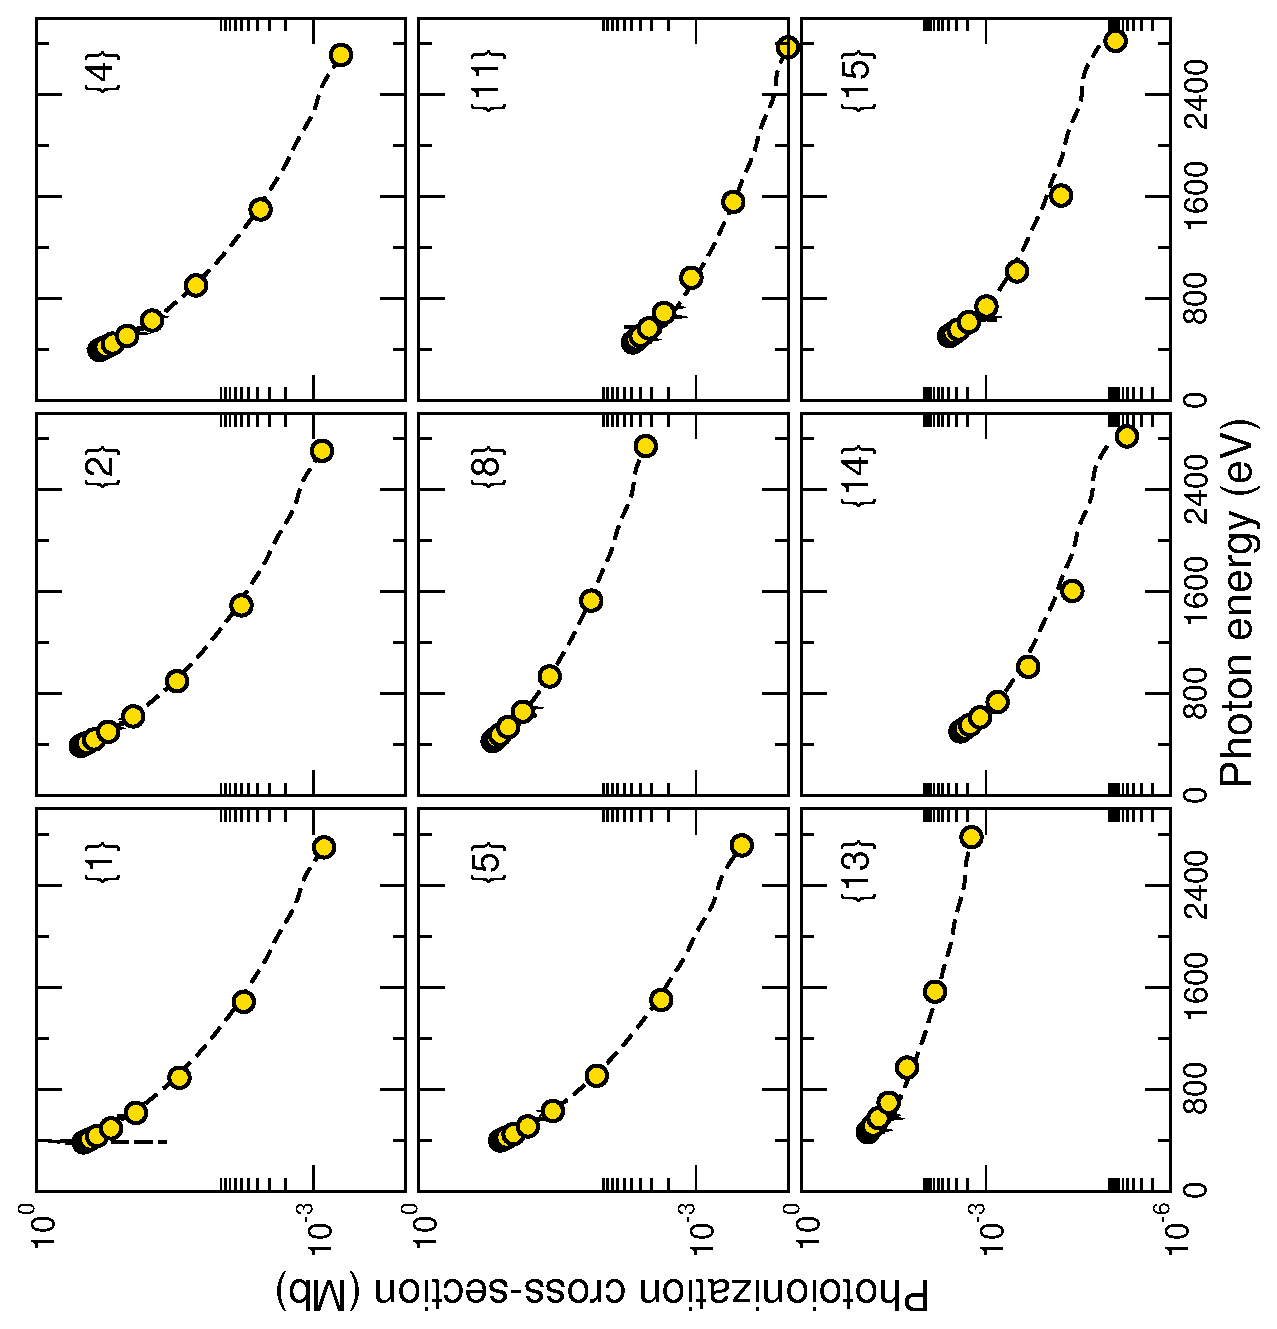
\includegraphics[scale=0.665, angle=-90]{Figures/Sulphur/open-adas/comparison3_new.eps}
\caption{Photoionization cross-sections presented on a logarithmic scale in Mb as a function of photon energy in eV up to 2,700 eV. Transitions are from the initial $^3$P$_0$ $\longrightarrow$ \{1\}, \{2\}, \{4\}, \{5\}, \{8\}, \{11\}, \{13\}, \{14\}, \{15\}. \label{fig:sul_adas0e}}
\end{figure}
%%%%
%%%
%%
%

We also present all possible comparisons with OPEN-ADAS for the lowest initial $^3$P split levels as a further measure of accuracy. A much larger energy mesh is adopted, as we consider just 500 equally spaced energy points across a range of 2,700 eV. This is the maximum energy we can achieve with the basis set employed. Figure \ref{fig:sul_adas2e} shows $^3$P$_2$ and Figures \ref{fig:sul_adas1e} and \ref{fig:sul_adas0e} contain the remaining $^3$P$_1$ and $^3$P$_0$ initial states respectively. We list the transitions within each of the captions, and for brevity, $\{$i$\}$ denotes the corresponding index in Table \ref{tab:sul_energy}. We see that excellent conformity is achieved for nearly all transitions but there are few discrepancies as expected from the two different approaches. The only major differences arise from Figure \ref{fig:sul_adas2e} and Figure \ref{fig:sul_adas1e} where the much weaker transitions are identified as h$\nu$ + $^3$P$_2$ $\rightarrow$ 2s2p$^4$ $^2$D$_{5/2}$ + e$^-$, and h$\nu$ + $^3$P$_1$ $\rightarrow$ 2s2p$^4$ $^2$D$_{3/2}$ + e$^-$ respectively, especially for the low energy region. 


                           %                                              %
                          %%%                                    %%%
       %%%%%%%%%%      SECTION     %%%%%%%%%%
                          %%%                                    %%%
                           %                                             %

\section{Resonance identification}
In this final Section we deal with the identification of the major resonant structure occurring due to autoionizing bound states arising from the indirect pathway scheme (\ref{eq:sul_process}). This identification can be achieved via the $QB$ technique as described in Section \ref{sec:rmat_qb}. We take $E_r$ as the energy position at resonance, $E_{n\rightarrow\infty}$ is the threshold in which each series converges to, and $z=9$. The limiting energy at $E_{n\rightarrow\infty}$ is taken simply as the target threshold value in Table \ref{tab:sul_energy}, which allows us to extract the quantum defects $\mu$ for each $E_r$ computed corresponding to equation (\ref{eq:rmat_qbdefect}). Resonance widths in this method are defined by equation (\ref{eq:rmat_qbwidth}), which incorporates the eigenphase sum and its energy derivative at the resonance position

%
%%
%%%
%%%%
\begin{figure}[hbt]
\includegraphics[scale=0.53, angle=-90]{Figures/Sulphur/threshold_single/threshold_single.eps}
\caption{Various photoionization cross-sections are presented on a logarithmic scale in Mb as a function of photoelectron energy given in eV. The first few resonances occur from the initial $LSJ$ states $^3$P$_2$, $^3$P$_1$, $^3$P$_0$, $^1$D$_2$ and $^1$S$_0$. We present the $J = 1$ odd resonance features and singular $J = 0$ odd resonance. \label{fig:sul_thresh}}
\end{figure}
%%%%
%%%
%%
%

A number of interesting resonance features appear clearly within the photoionization spectra displayed in Figures \ref{fig:sul_ground}, \ref{fig:sul_meta} and \ref{fig:sul_target}. In this Section we have identified the major contributors and estimate their widths in an intermediate coupling frame. There are obvious restrictions and limitations in displaying every resonance that has been identified, therefore only dominant contributions are considered.

%
%%
%%%
%%%%
\begin{sidewaysfigure}
\centering
\includegraphics[scale=0.85, angle=-90]{Figures/Sulphur/resonances/resonance1.eps}
\caption{The total ground state photoionization cross-section is presented on a logarithmic scale as a function of photon energy in eV. Presented are 2 major series that have common parent term $\Lambda_2$ and $\Lambda_3$ coupled to $l=2$ electrons and also the primary members of the $\Lambda_4$, $\Lambda_5$ and $\Lambda_8$ series. These are for select $J =1,2,3$ odd resonances exclusively. \label{fig:sul_resonances1}}
\end{sidewaysfigure}
%%%%
%%%
%%
%

%
%%
%%%
%%%%
\begin{sidewaysfigure}
\centering
\includegraphics[scale=0.85, angle=-90]{Figures/Sulphur/resonances/resonance2.eps}
\caption{The total ground state photoionization cross-section is presented on a logarithmic scale as a function of photon energy in eV. Presented are the resonances with common parent term $\Lambda_4$ and $\Lambda_5$ coupled to $l=2$ electrons and also primary members of the $\Lambda_6$ and $\Lambda_7$ series. These are for select $J =1,2,3$ odd resonances exclusively. \label{fig:sul_resonances2}}
\end{sidewaysfigure}
%%%%
%%%
%%
%

%
%%
%%%
%%%%
\begin{sidewaysfigure}
\centering
\includegraphics[scale=0.85, angle=-90]{Figures/Sulphur/resonances/resonance3.eps}
\caption{The total ground state photoionization cross-section is presented on a logarithmic scale as a function of photon energy in eV. Presented are the resonances with common parent term $\Lambda_6$, $\Lambda_7$ and also those of $\Lambda_8$ coupled to specific $l=1$ and $l=3$ electrons. These are for select $J =1,2,3$ odd resonances exclusively. \label{fig:sul_resonances3}}
\end{sidewaysfigure}
%%%%
%%%
%%
%


In order to convey these identifications visually, we divide the spectrum of Figure \ref{fig:sul_ground}, (depicting the ground state $^3$P$_2$ to the accessible $J=1, 2, 3$ odd states) into appropriate energy ranges. Each series of resonances that converges onto a single threshold we label to be $\Lambda_\zeta$ where the index is given in the first column of Table \ref{tab:sul_energy} and $\Lambda$ denoted as the parent term allocated to each $\zeta$. In our case, we consider those resonances up to and including convergence to the 8th threshold energy, $\Lambda_8 \equiv$ 2s2p$^4$ $^4$P$_{1/2}$.

Before beginning an extensive calculation, we are only required to analyse the ground state transition when considering the dominant $J=1, 2, 3$ odd state resonances. From Figure \ref{fig:sul_thresh}, all initial states of Figure \ref{fig:sul_ground} and Figure \ref{fig:sul_meta} are plotted as a function of photoelectron energy in eV. As expected, the $J = 1$ odd resonance ($\Gamma = 8.83$ meV) at $\approx 0.245$ eV is accessible through the initial states of $^3$P$_2$, $^3$P$_0$, $^1$S$_0$ and $^1$D$_2$. The much narrower $J = 0$ odd ($\Gamma = 0.19$ meV) resonance at $\approx 0.150$ eV however, is only accessible through the initial state of $^3$P$_1$. The remaining odd resonant states of $J = 0$ are omitted in this comparative work.

In Figure \ref{fig:sul_resonances1}, we present the first energy region of interest depicting major resonance series. Contained are the resonances belonging to [($\Lambda_2)nd$]$_{J=1}$ and [($\Lambda_3)nd$]$_{J=3}$ between an energy range of 382 - 392 eV. These resonances have been the most challenging in general to estimate due to an extremely crowded region of various autoionizing states. These resonances are studied in great detail and only accepted after every attempt has been made to rectify each identification. It is also possible to visualize lower members of series converging onto the thresholds of $\Lambda_4$, $\Lambda_5$ and even single contributors converging onto the $\Lambda_8$ threshold. The widths are not as easily identified for $\Lambda_4$ and $\Lambda_5$ within this energy window and therefore only the more pronounced isolated patterns are tabulated. 

Figure \ref{fig:sul_resonances2} contains resonances belonging to [($\Lambda_4)nd$]$_{J=1}$ and [($\Lambda_5)nd$]$_{J=2}$ between an energy range of 392 - 397 eV, along with early members of the $\Lambda_6$ and $\Lambda_7$ series. And finally, Figure \ref{fig:sul_resonances3} contains the remaining resonances belonging to [($\Lambda_6)np$]$_{J=2}$, [($\Lambda_7)np$]$_{J=2}$ and [($\Lambda_8)nf$]$_{J=2,3}$ between an energy range of 397 - 428 eV. We have also provided in Tables \ref{tab:sul_res1} and \ref{tab:sul_res2} a summary of energy positions, effective $n$, their quantum defects and line widths from all three Figures \ref{fig:sul_resonances1}, \ref{fig:sul_resonances2}, and \ref{fig:sul_resonances3} to visualise key trends.  Misidentifications are unfortunately unavoidable as seen from the narrow $\Gamma = 0.31$ meV and $\Gamma = 1.74$ meV widths of the [($\Lambda_2)14d$]$_{J=1}$ and  [($\Lambda_7)13p$]$_{J=2}$ series respectively and are enclosed by brackets within both tabulations. 

                           %                                              %
                          %%%                                    %%%
       %%%%%%%%%%      SECTION     %%%%%%%%%%
                          %%%                                    %%%
                           %                                             %
                           
\section{Conclusions}\label{se:sul_conclusions}
In this Section we summarize the results that we have obtained. We have initially implemented STO's to describe the one-electron spin orbitals of the form in equation (\ref{eq:many_boundorbs}). The tables of \citet{1974ADNDT..14..177C} provide an adequate description of $1s, 2s, 2p$ and then we have extended this to also include the $n = 3$ complex. This was accomplished by optimizing each $n = 3$ on their lowest lying energy term in $LS\pi$ coupling, using the computer package of {\sc civ3}. The 215 $J\pi$ target wavefunctions are generated by including 9 configurations in the close-coupling expansion, and a further 21 configurations to account for additional correlation in the wavefunctions. Energy levels of the S$^{9+}$ ion, produced by our present model, have been shown to be in excellent agreement with other theoretical values and observational measurements.
 
We have reported on a sophisticated study of the photoionization for the lowest five states of O-like S$^{8+}$. The photoionization spectra, evaluated using the {\sc bp} $R$-matrix method, have been properly delineated using a very fine mesh of photon energies, and an admirable agreement is found with the only other available data with which we can compare; the OPEN-ADAS database. This comparison between level resolved contributions is produced for the background cross-section only, and little disparity is evident for all photon energies considered. We have therefore benchmarked this semi-relativistic calculation, complete with autoionizing resonance features converging onto all target state thresholds.

Additionally, we have identified in the present analysis, through the $QB$ method, major resonance contributions and have tabulated their energy positions and linewidths alongside their quantum defects for each effective $n$. We believe our results presented here constitute the best and most accurate available to date given the sophistication of the model adopted and {\sc bprm} method used.



\begin{table}[hbt]
\footnotesize
\begin{center}
\begin{tabular}{@{} l c c c c @{}}
\toprule

\multicolumn{1}{c}{Resonance} & \multicolumn{1}{c}{$n$} & \multicolumn{1}{c}{E$_r$ (eV)} & \multicolumn{1}{c}{$\mu$} & \multicolumn{1}{c}{$\Gamma$ (meV)}  \\

\toprule
  \multicolumn{1}{c}{[$(\Lambda_2)nd]_{1}$} & 11 & 382.45 & 0.08 & 2.97 \\
  \multicolumn{1}{c}{} & 12 & 383.98 & 0.08 & 2.29  \\
  \multicolumn{1}{c}{} & 13 & 385.14 & 0.08 & 1.92  \\
  \multicolumn{1}{c}{} & (14) & (386.05) & (0.08) & (0.31)  \\
  \multicolumn{1}{c}{} & 15 & 386.78 & 0.08 & 1.13 \\
  \multicolumn{1}{c}{} & 16 & 387.38 & 0.08 & 0.93 \\
  \multicolumn{1}{c}{} & 17 & 387.88 & 0.08 & 0.65 \\
  \multicolumn{1}{c}{} & 18 & 388.31 & 0.08 & 0.64 \\
  \multicolumn{1}{c}{} & $\vdots$ & $\vdots$ & $\vdots$ & $\vdots$ \\
  \multicolumn{1}{c}{} & $\rightarrow \infty$ & 391.74 & $\cdots$ & $\cdots$ \\
                                     \midrule
   \multicolumn{1}{c}{[$(\Lambda_3)nd]_{3}$} & 11 & 382.70 & 0.09 & 4.05 \\
  \multicolumn{1}{c}{}  & 12 & 384.20 & 0.08 & 3.62 \\
  \multicolumn{1}{c}{}   & 13 & 385.34 & 0.09 & 2.34 \\
  \multicolumn{1}{c}{} & 14 & 386.27 & 0.09 & 1.78 \\
 \multicolumn{1}{c}{}  & 15 & 387.00 & 0.09 & 1.43 \\
 \multicolumn{1}{c}{}   & 16 & 387.60 & 0.09 & 1.21 \\
 \multicolumn{1}{c}{}  & 17 & 388.10 & 0.09 & 0.94 \\
 \multicolumn{1}{c}{}  & 18 & 388.51 & 0.09 & 0.76 \\
  \multicolumn{1}{c}{}  & $\vdots$ & $\vdots$ & $\vdots$ & $\vdots$ \\
  \multicolumn{1}{c}{}  & $\rightarrow \infty$ & 28.808 & $\cdots$ & $\cdots$ \\
                               \midrule
  \multicolumn{1}{c}{[$(\Lambda_4)nd]_{1}$} & 15 & 391.98 & 0.06 & 1.43  \\
  \multicolumn{1}{c}{} & 16 & 392.59 & 0.06 & 1.21  \\
  \multicolumn{1}{c}{} & 17 & 393.08 & 0.06 & 1.10  \\
  \multicolumn{1}{c}{} & 18 & 393.50 & 0.06 & 0.83  \\
  \multicolumn{1}{c}{} & 19 & 393.86 & 0.06 & 0.69  \\
  \multicolumn{1}{c}{} & 20 & 394.16 & 0.06 & 0.61  \\
  \multicolumn{1}{c}{} & 21 & 394.42 & 0.05 & 0.57  \\
  \multicolumn{1}{c}{} & 22 & 394.63 & 0.07 & 0.44 \\
  \multicolumn{1}{c}{} & $\vdots$ & $\vdots$ & $\vdots$ & $\vdots$  \\
  \multicolumn{1}{c}{} & $\rightarrow \infty$ & 396.92 & $\cdots$ & $\cdots$   \\
                    \midrule
   \multicolumn{1}{c}{[$(\Lambda_5)nd]_{1}$} & 15 & 392.25 & 0.04 & 1.61 \\
  \multicolumn{1}{c}{}   & 16 & 392.84 & 0.04 & 1.33 \\
  \multicolumn{1}{c}{}   & 17 & 393.34 & 0.04 & 1.10 \\
  \multicolumn{1}{c}{}  & 18 & 393.75 & 0.04 & 0.94 \\
  \multicolumn{1}{c}{}  & 19 & 394.09 & 0.05 & 0.79 \\
  \multicolumn{1}{c}{}  & 20 & 394.40 & 0.06 & 0.68 \\
  \multicolumn{1}{c}{} & 21 & 394.68 & 0.04 & 0.57 \\
  \multicolumn{1}{c}{}   & 22 & 394.87 & 0.04 & 0.50  \\
  \multicolumn{1}{c}{}   & $\vdots$ & $\vdots$ & $\vdots$ & $\vdots$ \\
  \multicolumn{1}{c}{}  & $\rightarrow \infty$ & 397.18 & $\cdots$ & $\cdots$ \\
           
  
                    
                                                   \bottomrule
 \end{tabular}
 \caption{Dominant resonances [$(\Lambda_2)nd]_{{\rm J=1}}$ and [$(\Lambda_3)nd]_{{\rm J=3}}$ between the energy range of 382.3 - 393.2 eV and, [$(\Lambda_4)nd]_{{\rm J=1}}$ and [$(\Lambda_5)nd]_{{\rm J=1}}$ between the energy range of 391.8 - 397.3 eV originating from the 2s$^2$2p$^4$ $^3$P$_2$ initial state are presented. We present the resonance energy $E_r$, given in eV, the effective quantum number $n$, the quantum defects $\mu$ and decreasing line widths $\Gamma$ displayed in units of meV. $E_{n\rightarrow \infty}$ are taken from Table \ref{tab:sul_energy} and all data is generated from the {\sc qb} code. \label{tab:sul_res1}}
 \end{center}
\end{table}


\begin{table}[h]
\footnotesize
\begin{center}
\begin{tabular}{@{} l c c c c @{}}
\toprule

\multicolumn{1}{c}{Resonance} & \multicolumn{1}{c}{$n$} & \multicolumn{1}{c}{E$_r$ (eV)} & \multicolumn{1}{c}{$\mu$} & \multicolumn{1}{c}{$\Gamma$ (meV)}  \\

\toprule
        
  \multicolumn{1}{c}{} & 6 & 394.76 & 0.24 & 21.22  \\        
  \multicolumn{1}{c}{[$(\Lambda_6)np]_{2}$} & 7 & 403.84 & 0.23 & 16.60\\
  \multicolumn{1}{c}{} & 8 & 409.65 & 0.23 & 11.93  \\
  \multicolumn{1}{c}{} & 9 & 413.59 & 0.23 & 9.48  \\
  \multicolumn{1}{c}{} & 10 & 416.36 & 0.23 & 6.73  \\
  \multicolumn{1}{c}{} & 11 & 418.42 & 0.23 & 5.16  \\
  \multicolumn{1}{c}{} & 12 & 419.95 & 0.23 & 4.18  \\
  \multicolumn{1}{c}{} & 13 & 421.15 & 0.23 & 2.04  \\
  \multicolumn{1}{c}{} & $\vdots$ & $\vdots$ & $\vdots$ & $\vdots$ \\
  \multicolumn{1}{c}{} & $\rightarrow \infty$ & 427.91 & $\cdots$ & $\cdots$ \\
           \midrule
          \multicolumn{1}{c}{}  & 6 & 395.67 & 0.23 & 19.59 \\        
  \multicolumn{1}{c}{[$(\Lambda_7)np]_{2}$} & 7 & 404.72 & 0.23 & 18.10 \\
  \multicolumn{1}{c}{}  & 8 & 410.48 & 0.23 & 11.28 \\
  \multicolumn{1}{c}{} & 9 & 414.42 & 0.22 & 8.33 \\
  \multicolumn{1}{c}{}  & 10 & 417.19 & 0.22 & 5.67 \\
  \multicolumn{1}{c}{}  & 11 & 419.23 & 0.22 & 4.07 \\
  \multicolumn{1}{c}{} & 12 & 420.77 & 0.23 & 2.93 \\
  \multicolumn{1}{c}{} & (13) & (421.97) & (0.23) & (1.74) \\
  \multicolumn{1}{c}{} & $\vdots$ & $\vdots$ & $\vdots$ & $\vdots$ \\
  \multicolumn{1}{c}{} & $\rightarrow \infty$ & 428.72 & $\cdots$ & $\cdots$ \\
           \midrule
  \multicolumn{1}{c}{} & 5 & 384.93 & 0.01 & 45.17  \\        
  \multicolumn{1}{c}{[$(\Lambda_8)nf]_{2}$} & 6 & 398.44 & 0.01 & 15.65  \\
  \multicolumn{1}{c}{} & 7 & 406.59 & 0.01 & 14.56  \\
  \multicolumn{1}{c}{} & 8 & 411.89 & 0.01 & 9.48  \\
  \multicolumn{1}{c}{} & 9 & 418.10 & 0.01 & 6.46  \\
  \multicolumn{1}{c}{} & 10 & 420.02 & 0.01 & 4.59  \\
  \multicolumn{1}{c}{} & 11 & 421.49 & 0.01 & 3.36 \\
  \multicolumn{1}{c}{} & 12 & 422.62 & 0.01 & 2.61 \\
  \multicolumn{1}{c}{} & $\vdots$ & $\vdots$ & $\vdots$ & $\vdots$ \\
  \multicolumn{1}{c}{} & $\rightarrow \infty$ & 31.542 & $\cdots$ & $\cdots$ \\
                        \midrule
            \multicolumn{1}{c}{} &  5 & 384.95 & 0.01 & 40.00 \\        
  \multicolumn{1}{c}{[$(\Lambda_8)nf]_{3}$} & 6 & 398.44 & 0.01 & 19.32 \\
  \multicolumn{1}{c}{}  & 7 & 406.59 & 0.01 & 12.10 \\
  \multicolumn{1}{c}{}  & 8 & 411.89 & 0.01 & 7.74 \\
  \multicolumn{1}{c}{} & 9 & 418.10 & 0.01 & 5.21 \\
  \multicolumn{1}{c}{}  & 10 & 420.02 & 0.01 & 3.69 \\
  \multicolumn{1}{c}{}   & 11 & 421.49 & 0.01 & 2.67 \\
  \multicolumn{1}{c}{}   & 12 & 422.62 & 0.01 & 2.12 \\
  \multicolumn{1}{c}{} & $\vdots$ & $\vdots$ & $\vdots$ & $\vdots$ \\
  \multicolumn{1}{c}{} & $\rightarrow \infty$ & 429.15 & $\cdots$ & $\cdots$ \\
                                                   \bottomrule
 \end{tabular}
 \caption{Dominant resonances [($\Lambda_6)np$]$_{J=2}$, [($\Lambda_7)np$]$_{J=2}$, and [($\Lambda_8)nf$]$_{J=2,3}$ between the energy range of 397.2 - 429.9 eV and with single identifications of each series within the lower energy range of 394.5 - 395.9 eV and at $\approx$ 384.9 Ryd originating from the 2s$^2$2p$^4$ $^3$P$_2$ initial state are presented. We present the resonance energy $E_r$, given in Ryd, the effective quantum number $n$, the quantum defects $\mu$ and decreasing line widths $\Gamma$ displayed in units of meV. $E_{n\rightarrow \infty}$ are taken from Table \ref{tab:sul_energy} and all data is generated from the {\sc qb} code. \label{tab:sul_res2}}
 \end{center}
\end{table}


%----------------------------------------------------------------------------------------


